

\subsection{Double Blast Test}

Two interacting blast waves on a 1-dimensional grid. This test is very difficult to solve on an Eulerian grid due to the 
strong shocks and multiple interactions with rarefactions and contact discontinuities, and is useful in measuring a 
solver's ability to handle these types of events. 

\subsubsection{Analysis}

The two blast waves propogate toward one another and collide, producing more contact discontinuities.
Could calculate the exact time they collide. Solve sod problem.

\begin{figure*}
\begin{center}
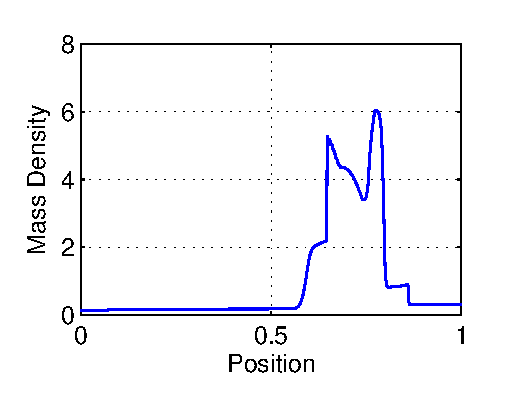
\includegraphics{DoubleBlast.eps}
\caption{Double Blast at t = 0.038}
\end{center}
\end{figure*}
\subsubsection{Initial Conditions}

Boundary conditions are mirrored around the X axis and periodic everywhere else.

The physical input parameters to the double blast test are:
\begin{itemize}
\item \tt{Pl} - Sets the pressure of the blastwave originating in the left-most tenth of the grid
\item \tt{Pr} - Similarly sets the pressure of the right-most blastwave
\item \tt{Pa} - Sets the ambient pressure
\end{itemize}


with the initial conditions set by each of the three zones being defined as an adiabatic gas with $\gamma$ = 1.4 everywhere. 
We set $\tt{Pl} = 1000$, $\tt{Pr} = 100$, and $\tt{Pa} = 0.01$. Initial momenta are zero everywhere.
